\documentclass[informe.tex]{subfiles}
\begin{document}

\textbf{Datos del filtro}	\newline	
								
	\begin{tabular}{ |c | c| c| c|}
		\hline
			 Tipo     & Pasa bajo &  Chebyshev &  IIR \\
 			 Hardware & Microcontrolador & STM32F407 & \\		
			$ f_m $  & 22418  & Hz & Frecuencia de muestreo \\
			$ f_c $  & 1000   & Hz & Frecuencia de corte (3dB) \\
			$ f_p $  & 950    & Hz & Frecuencia en la banda de paso\\
			$ A_p $  & 0.1    & dB & Atenuación en la banda de paso \\			
			$ f_s $  & 1150   & Hz & Frecuencia en la banda de rechazo \\
			$ A_s $  & 15     & dB & Atenuación en la banda de rechazo \\
			$ N $   & 8      &  & Orden del filtro necesario \\			
		\hline
	\end{tabular}\newline\newline		
	
\textbf{Función de transferencia del filtro analógico}\newline
	\begin{tiny}
		\subfile{../design_matlab/output/stm32_iir_lp_chebyshev_ecu_s.tex}
	\end{tiny}\newline
    	
    	\underline{Función de transferencia del filtro digital}\newline
	\begin{tiny}
		\subfile{../design_matlab/output/stm32_iir_lp_chebyshev_ecu_z.tex}
	\end{tiny}\newline
	
\textbf{Respuesta en frecuencia}\newline
	\begin{tabular}{p{0.5\textwidth} p{0.5\textwidth}}		
		\begin{wrapfigure}{l}{0.9\linewidth}
    		\centering
    		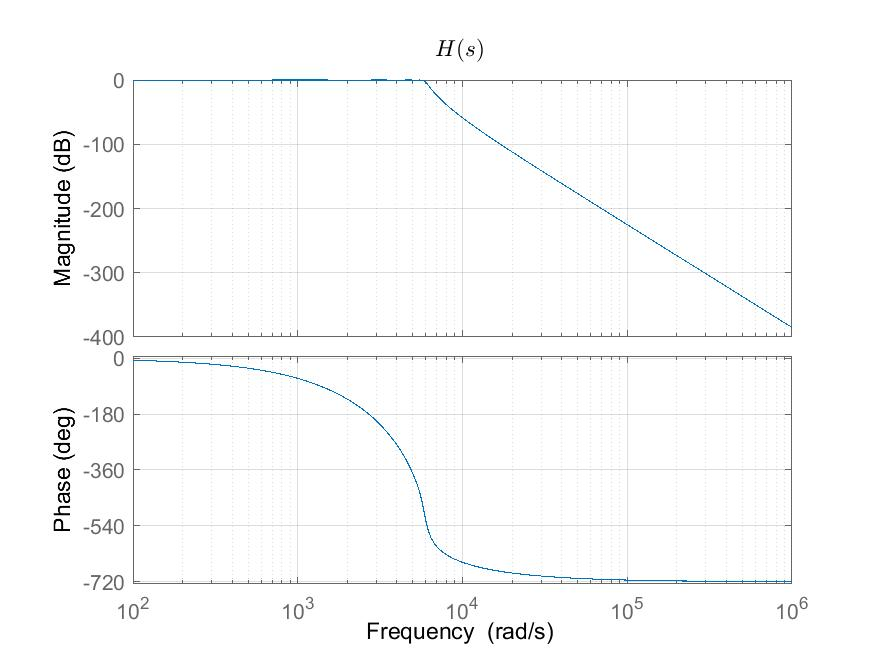
\includegraphics[width=\linewidth]{stm32_iir_lp_chebyshev_2.jpg}
    		\caption{Filtro analógico}
		\end{wrapfigure}					
		&	
	 	\begin{wrapfigure}{l}{0.9\linewidth}
    		\centering
    		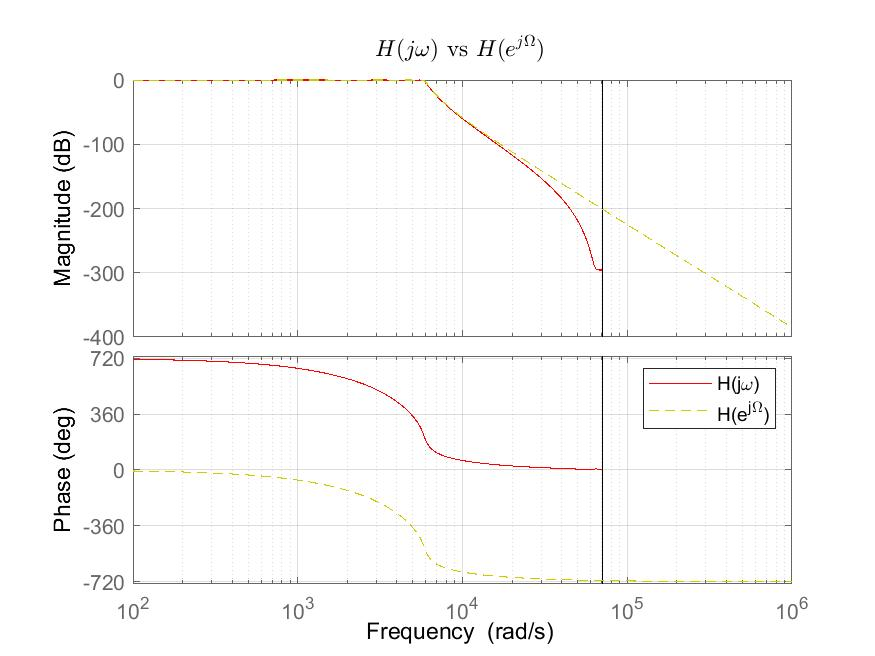
\includegraphics[width=\linewidth]{stm32_iir_lp_chebyshev_6.jpg}
    		\caption{Filtro digital}
		\end{wrapfigure}			
	 	\\ 
	\end{tabular}\newpage
	
\textbf{Diagrama de Polos y ceros}\newline
	\begin{tabular}{p{0.5\textwidth} p{0.5\textwidth}}		
		\begin{wrapfigure}{l}{0.9\linewidth}		
    		\centering
    		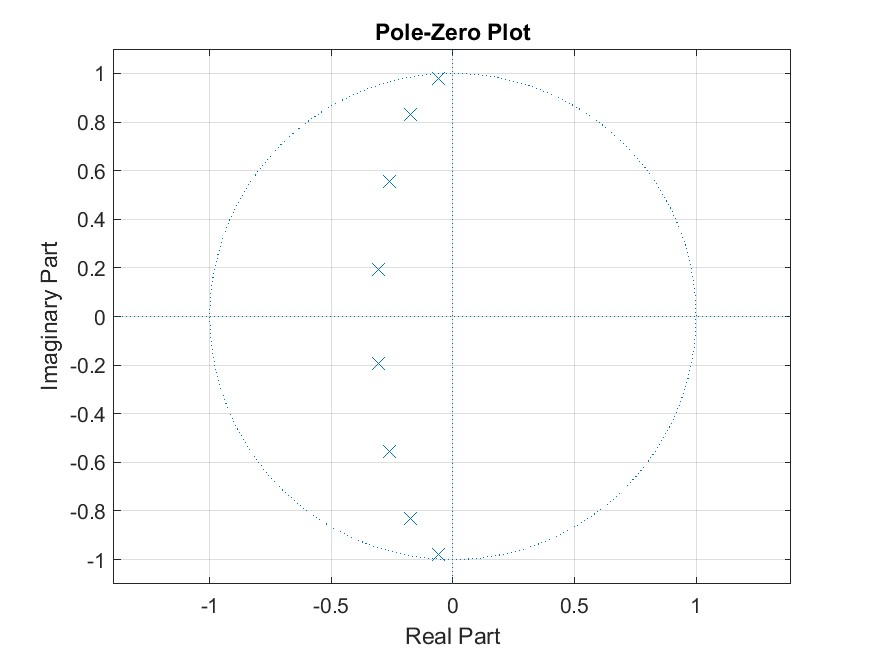
\includegraphics[width=\linewidth]{stm32_iir_lp_chebyshev_1.jpg}
    		\caption{Filtro Analógico}
		\end{wrapfigure}					
		&	
	 	\begin{wrapfigure}{l}{0.9\linewidth}
    		\centering
    		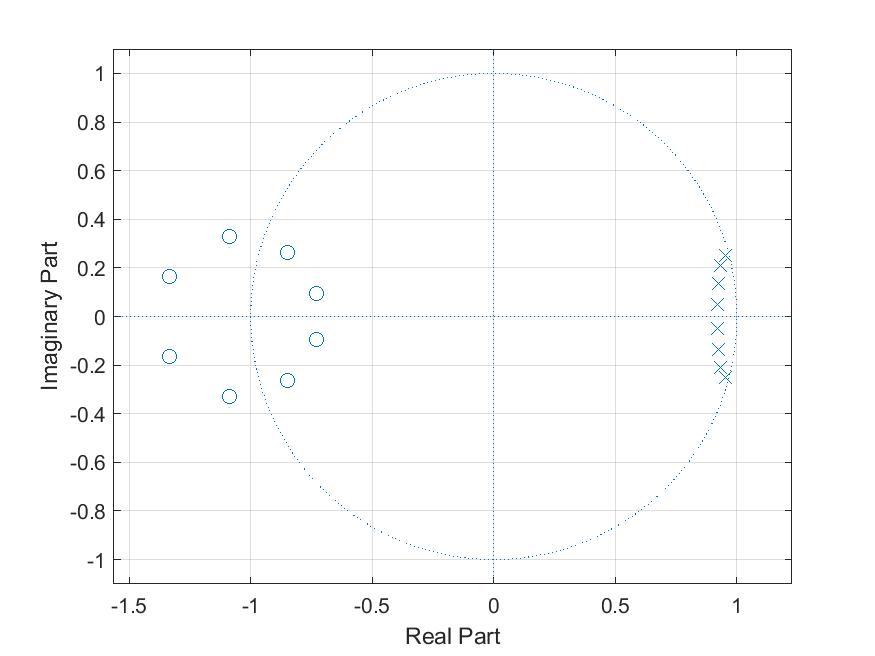
\includegraphics[width=\linewidth]{stm32_iir_lp_chebyshev_5.jpg}
    		\caption{Filtro Digital}
		\end{wrapfigure}			
	 	\\ 
	\end{tabular}\newline\newline\newline\newline\newline\newline\newline\newline\newline\newline\newline\newline\newline 	\newline\newline\newline\newline\newline\newline

\textbf{Coeficientes preparados para el microcontrolador}\newline

\lstinputlisting[language=c, frame=single]{../design_matlab/output/stm32_iir_lp_chebyshev_stm32_coef.txt}
	
\end{document}